\documentclass[12pt]{extarticle}
\usepackage[T1]{fontenc}
\usepackage[utf8]{inputenc}
\usepackage{charter, graphicx}
\usepackage{environ}
\usepackage{indentfirst}
\usepackage{lipsum} % for dummy text
% \usepackage{enumitem}
\usepackage[a4paper, total={6.5in, 10in}]{geometry}
% \usepackage{minted}
% \usepackage[T1]{fontenc}
% \usepackage{textcomp}
% \usepackage[scaled]{beramono}

\usepackage{biblatex}
\usepackage{caption}
\usepackage{subcaption}

\usepackage[colorlinks,citecolor=green,urlcolor=blue]{hyperref}
\addbibresource{./sample.bib} 
\title{Probabilistic Programming in Multicore OCaml}
\author{Arnhav Datar, CS18B003\\Dr. KC Sivaramakrishnan}
\date{January 2021}

\begin{document}

\maketitle

\section*{Research Problem}

Probabilistic programming languages(PPLs) are used for performing Bayesian inference \cite{Baydin_2019} in complex generative models. 
Probabilistic Programming \cite{vandemeent2018introduction} involves the construction of inference problems and the development of corresponding evaluators, that computationally characterize the denoted conditional distribution.

Probabilistic programming has shown applications \cite{appl} in the fields of computer vision, cryptography, quantitative finance, biology and reliability analysis. 
Given the recent rise of probabilistic programming for academic and industry use, we aim to make a Probabilistic Programming Library in Multicore OCaml. 

% \subsection*{Effect Handlers}
% Effect Handlers\cite{effects} allow us to handle algebraic effects (in a way similar to exception handlers with exceptions). Multi-Core OCaml currently has support for algebraic effect handlers as a way of supporting concurrency primitives. A use of algebraic effect handlers is given below.
% \begin{listing}[H]\centering
% \begin{minted}[linenos]{ocaml}
% effect foo: int -> int
% let f() = 1 + (perform (foo 3))
% let r =
%     try f()
%     with effect (foo i) k -> continue k (i+1)
% \end{minted}
% \caption{Demonstrating Effect Handlers in Multi-Core OCaml}
% \end{listing}
% \noindent
% \textbf{Control Flow of the above program}
% \begin{enumerate}[topsep=1pt,itemsep=2pt, parsep=2pt]
%     \item Function f() is tried and it encounters the perform
%     \item Upon seeing the perform is jumps to the effect portion. 
%     \item Here is substitutes the value of 3 in i and returns 4 to function. 
%     \item Here k is a continuation point to keep track of the function from where we jumped from and then we finally return the value 4 to the function.
%     \item finally the value 5 is return from f() and given to r.
% \end{enumerate}

%  For seeing further examples of effect handlers in multi-core OCaml refer \cite{ocaml-multicore}. Effect handlers have been used for probabilistic programming languages\cite{hack, pyro}. Clearly effect handlers coalesce very well with probabilistic programming, our project will delve into the same in Multi-Core OCaml. 

% \section*{Motivation}
OCaml is becoming very popular in various applications such as advanced financial management, transparency of global financial markets, phylogenetic inference, social media innovations etc. 
Absence of concurrent probabilistic programming libraries in OCaml is putting limitations on the usage. Given that the inferences done in probabilistic programming can be computationally heavy, the library will be a valuable resource for the OCaml community. 

% \section*{Hypothesis}

Until recently, probabilistic programming was limited in scope, and most inference algorithms had to be written manually for each task. 
Recently with availability of higher computing power and advances in concurrency, the probabilistic programming is becoming ubiquitous. 
To support the higher computational demand and to improve the performance we would like to explore effect handlers in Multicore OCaml to implement concurrent algorithms. 
 
 
\section*{Literature Review}

There have been many probabilistic programming efforts both as libraries and as independent languages. 
The development of these languages has sped up in the past few years, there being a lot of languages/libraries developed in the last 5 years. 
Some noteworthy mentions are Stan\cite{stan}, Pyro\cite{pyro}, HackPPL\cite{hack}, CuPPL\cite{collins2020probabilistic}, OwlPPL\cite{roy2020probabilistic} and LF-PPL\cite{zhou2019lfppl}. 

To the best of our knowledge the following probabilistic programming works are associated with OCaml and effect handlers. IBAL \cite{IBAL} and Hansei \cite{Hansei} were PPLs which were implemented in OCaml. 
However the languages weren't universal languages. Universal probabilistic languages can have an unlimited number of random variables. 
Furthermore they are not implemented using effect handlers and they aren't parallelised.

More recently Anik Roy made a universal PPL using Owl\cite{wang2018owl}(a general-purpose numerical library in OCaml) known as OwlPPL\cite{roy2020probabilistic}, however it did not use effect handlers, like its predecessors. 
It used a variety of inference algorithms ranging from simple enumeration to MCMC methods like Metropolis-Hastings. 
% \begin{enumerate}
%     \item Rejection Sampling
%     \item Importance Sampling
%     \item Metropolis Hastings
%     \item Particle Cascade
%     \item Particle Filter
%     \item Particle Independent Metropolis-Hastings
% \end{enumerate}
 While these algorithms are properly implemented and analysed, it does not include more recent successful inference algorithms like the Hamiltonian Monte Carlo\cite{betancourt2018conceptual} and the No U-Turn Sampler\cite{hoffman2011nouturn}.  
 
 Effect handlers have been used for developing modern universal PPLs like Hack-PPL\cite{hack} (Facebook's PPL) and Pyro\cite{pyro}(Uber's PPL). Pyro was built on Poutine which is a library of Effect handlers. However Hack-PPL is a separate programming language and Pyro is a library in Python/Pytorch. Edward\cite{tran2017deep} is a modern probabilistic modelling library that supports concurrency, but it does not use effect handlers(uses Tensorflow) and is not universal.

 Multicore OCaml currently has support for algebraic effect handlers as a way of supporting concurrency primitives. In this project we propose to modify Anik Roy's OwlPPL to add other recent concurrent inference algorithms. 
 %such as the Hamiltonian Monte Carlo and the No U-Turn Sampler. We further propose to parallelise the other inference algorithms present in OwlPPL.
 %Algebraic Effect Handlers\cite{ocaml-multicore, effects} allow us to handle algebraic effects (in a way similar to exception handlers with exceptions). 


\section*{Timeline}
\noindent

Given below is rough Gantt Timeline for the project. As can be seen we have divided the work in segments of coding, learning, testing, evaluation and report writing. Each section has 2-3 subsections. 
\begin{figure}[!htb]
    \centering
    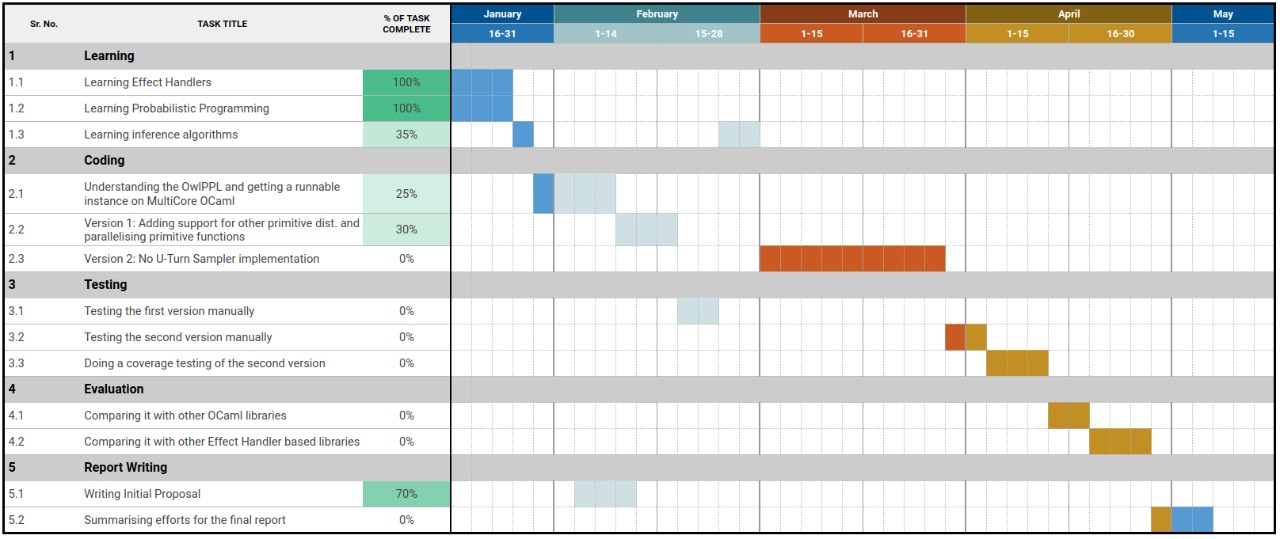
\includegraphics[width=\textwidth]{./images/gantt2.jpeg}
    \caption{Brief Timeline, A column represents roughly 3 days}
    \label{fig:my_label}
\end{figure}

% till Feb complete reading and planning\\
% February - Make a simple model with a simple inference algorithm and test it\\
% March - Learn various inference algorithms and start adding them to the code\\
% April - Start testing manually and do a code coverage checks, also start evaluating performance of the code compared to other libraries.\\ 
% May - Create report summarising findings. 

Currently OwlPPL has support for only 8 primitive distributions. These are binomial, normal, categorical, uniform(Discrete and Continuous), beta, gamma and Bernoulli. This is significantly lower than most other libraries. We will first remedy this as well as go through the code in the initial phases of the project. For implementing the primitive distributions we intend to use Owl\cite{wang2018owl}, wherever possible. We will also try to make other primitive functions like sample\_n( a function which returns n samples from a distribution) concurrent. We will do a manual testing of the code so far at this point. 

Following this we will implement the No-U-Turn Sampler\cite{hoffman2011nouturn} with the leap-frog integrator,  using Effect Handlers. This is the main portion of the project and will therefore take a significant amount of time.  The choice of No-U Turn sampler is based on the fact that it is parallelisable and has shown promising results in converging to the required value/distribution. Furthermore most of the modern PPLs(Stan, Pyro, Hack-PPL et.al.) have used this sampler.  

If we seem to be going ahead of schedule, we would try to implement the original inference algorithms in the OwlPPL library using effect handlers. Some of the algorithms like the particle cascade can clearly be parallelised. However algorithms like the Metropolis Hastings is a Markov Chain Monte Carlo, hence making it difficult to be parallelised. 


%  We then propose to add atleast one of the two inference algorithms which are being heavily used in literature nowadays
%  \begin{enumerate}
%      \item Hamiltonian Sampler 
%      \item No U-Turn Sampler
%  \end{enumerate}
 
%  We give a higher preference to the No U-Turn sampler. While its harder to implement, modern PPLs(eg: Stan and Pyro) use this sampler. However the two samplers are reasonably similar. 
 
 We will post this stage do a manual as well as coverage testing of the algorithms implemented. We will then move on to evaluating the performance of our library to other similar works for some benchmarks. These benchmarks will test performance on single core as well as multiple cores, and will also test the performance based on number of samples. 



% Initially we will build a simple enumeration inference algorithm by February end. This will be manually tested. It will also have a variety of primitive distributions(both discrete and continuous). We will then proceed to implementing other algorithms and testing them. We will finally conclude with testing and evaluating performance against some of the other probabilistic programming libraries/languages described in the literature review.



% \section*{Deliverable}
% We intend to build a library for universal probabilistic programming in Multicore OCaml with reasonable performance using effect handlers. We will try to implement atleast two inference algorithms for the same, as time permits. If we are successful, this may lead to a workshop paper. The performance of our library should preferably surpass other OCaml libraries in a multicore setting. 
\printbibliography
\end{document}
